\section{分类问题}
\subsection{由回归到分类}
对于二元分类问题,一个自然的想法是当做回归问题求解,对于一类样本,令函数目标值为1,另一类目标值为-1。这在两类样本分布合理情况下是可以做到的,但是当样本分布差异很大时,从回归的角度思考就会出现问题。如图\ref{fig:ref_to_classification}所示:
\begin{figure}[ht]
	\centering
	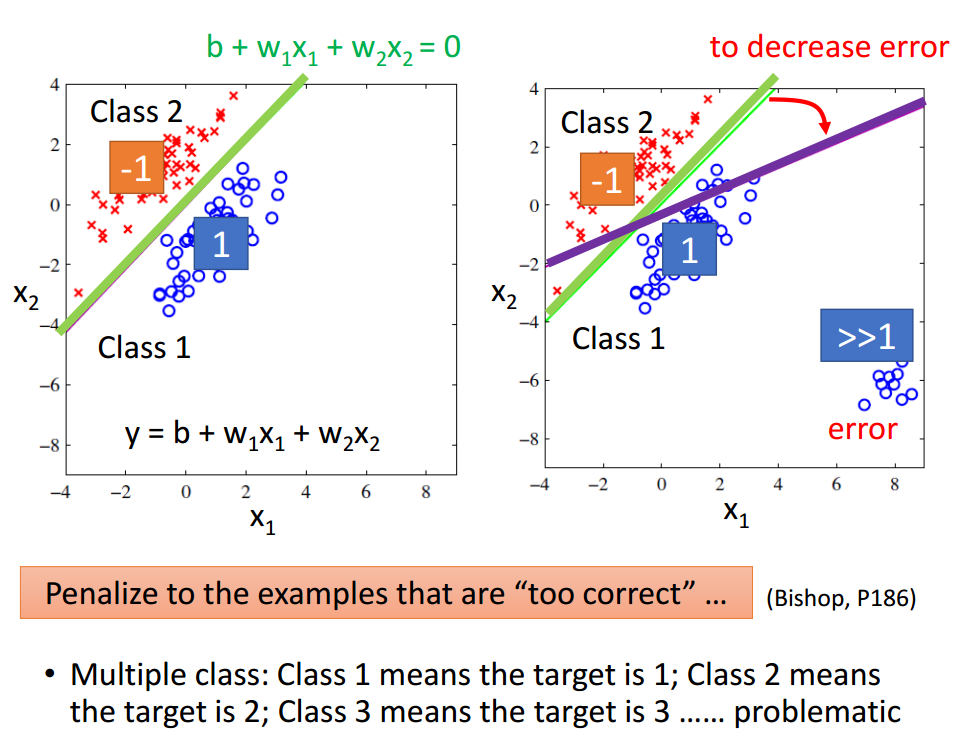
\includegraphics[scale=0.5]{pic/regression_to_classification.png}
	\caption{不合理的分布导致回归求解分类问题时出错}
	\label{fig:ref_to_classification}
\end{figure}
右下角的异常点导致回归得到边界线是紫色线,出现错误。而对于多类分类问题,依旧尝试使用回归求解,如类别1、2、3分别赋予目标值1、2、3则是不行的。

\subsection{概率论基础知识}
\begin{myquotation}{贝叶斯准则:}
\begin{description}
	\item[加和规则] $p(X)=\sum_Y p(X,Y)$
	\item[乘积规则] $p(X,Y)=p(Y|X)p(X)$
\end{description}
\end{myquotation}

考虑随机变量$X$和$Y$,如图\ref{fig:Bayesian lawl}所示:
\begin{figure}[ht]
	\centering
	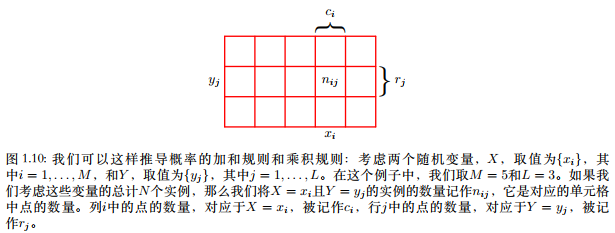
\includegraphics[scale=0.5]{pic/gailv}
	\caption{贝叶斯准则}
	\label{fig:Bayesian lawl}
\end{figure}
$X=x_i$且$Y=y_j$ 的联合概率:
\[
p(X=x_i,Y=y_j)=\frac{n_ij}{N}
\]
$X=x_i$ 的概率:
\[
p(X=x_i)=\frac{c_i}{N}=\frac{\sum_{j=0}^L n_{ij}}{N}=\frac{\sum_{j=0}^L p(X=x_i,Y=y_j)*N}{N}=\sum_{j=0}^L p(X=x_i,Y=y_j)
\]
上述公式,即为\emph{加和规则}。$p(X=x_i)$ 也称为边缘概率。
\[
p(X=x_i,Y=y_j)=\frac{n_{ij}}{N}=\frac{n_{ij}}{c_i} \frac{c_i}{N}=p(Y=y_j|X=x_i)p(X=x_i)
\]
称为概率的\emph{乘积规则}。
\[
p(X,Y)=p(Y|X)P(X)=p(Y,X)=p(X|Y)p(Y)
\]
则:
\begin{equation}
p(Y|X)=\frac{p(X|Y)p(Y)}{p(X)}=\frac{p(X|Y)p(Y)}{\sum_Y{p(X,Y)}}=\frac{p(X|Y)p(Y)}{\sum_Y{p(X|Y)p(Y)}}
\end{equation}

贝叶斯定理:$Y$ 对 $X$ 的条件概率可由 $X$ 对 $Y$ 的条件概率计算得到。

\subsection{二分类问题}

\subsubsection{生成模型 Generative}

考虑盒子和蓝绿球,如图\ref{fig:green_blue_ball}:
\begin{figure}[ht]
	\centering
	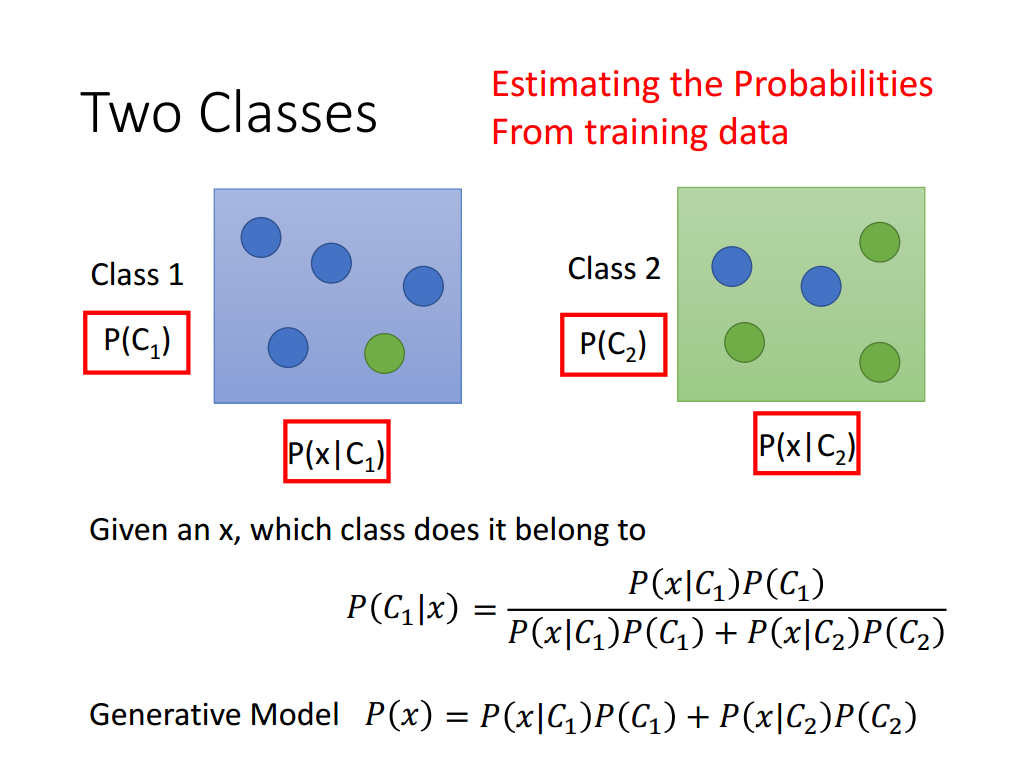
\includegraphics[scale=0.4]{pic/classification_01}
	\caption{蓝绿球概率问题}
	\label{fig:green_blue_ball}
\end{figure}
现抽一个绿球,求该球来自于class 1的概率$P(C_1|x)$:可通过贝叶斯定理求出。

这是生成模型的思想,学习的是模型,如上图\ref{fig:green_blue_ball}中,分别学习两个类别的模型,$p(x|C_1),p(x|c_2)$来求得新样本属于类别的概率:$p(C|x)$ 。实质上,生成模型学习的是联合概率$p(X,Y)$ 。分子部分$p(x|C_1)p(C_1)$

考虑这样一个例子,假设给定动物的若干个特征属性,我们希望通过这些特征学习给定的一个“个体”到底是属于“大象”($y=1$)还是“狗”($y=0$)。如果采用判别模型的思路,如逻辑回归,我们会根据训练样本数据学习类别分界面,然后对于给定的新样本数据,我们会判断数据落在分界面的哪一侧从而来判断数据究竟是属于“大象”还是属于“狗”。在这个过程中,我们并不会关心,究竟“大象”这个群体有什么特征,“狗”这个群体究竟有什么特征。

现在我们来换一种思路,我们首先观察“大象”群体(training data),我们可以根据“大象”群体特征建立模型,然后再观察“狗”群体特征,然后再建立“狗”的模型。当给定新的未知个体时,我们将该个体分别于“大象”群体和“狗”群体模型进行概率比较,看这个个体更符合哪个群体模型的特征。

核心的方法是对于同一类数据,假定服从一种分布,如高斯分布,对于新的样本,计算其属于不同类别的分布的概率。

对于一类训练样本,计算特征均值和方差矩阵,通过下式计算概率:
$$f_{\mu,\Sigma}=\frac{1}{(2\pi)^{D/2}} \frac{1}{|\Sigma|^{1/2}} \exp \left\{-\frac{1}{2} (x-\mu)^T \Sigma^{-1} (x-\mu)\right\}$$

通常,不同类别的$\Sigma$选取一样,以防止过拟合,此时模型为线性的,对于二维特征,样本分界面是一条直线。
\begin{figure}[ht]
	\centering
	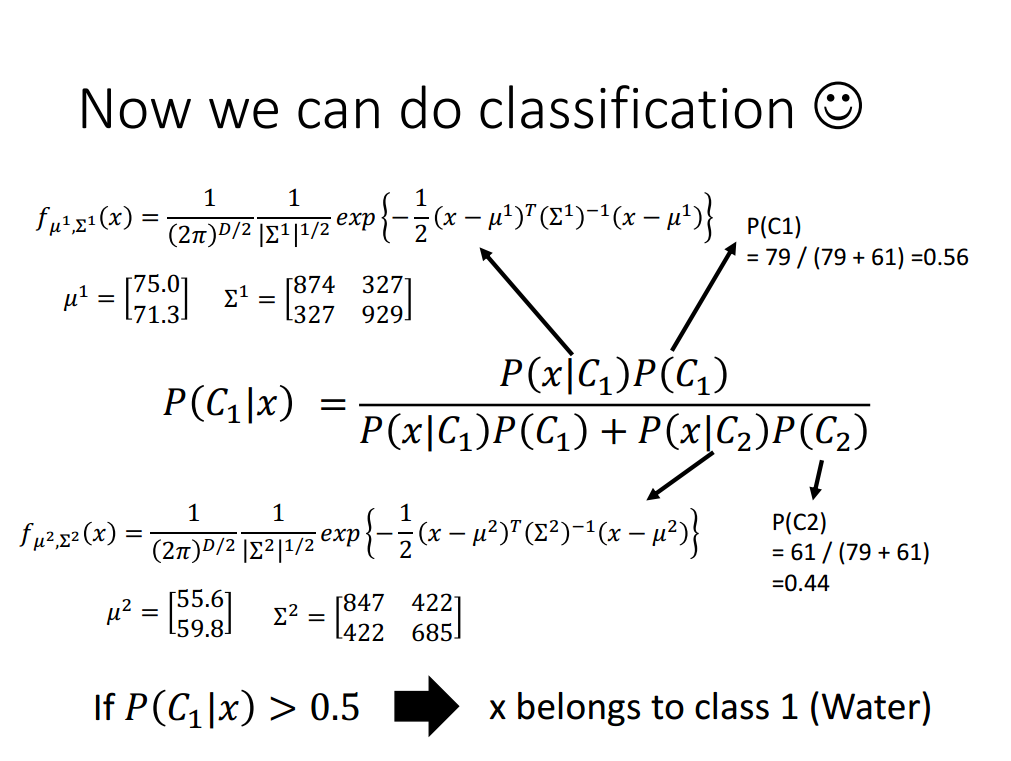
\includegraphics[scale=0.4]{pic/generative_model}
	\caption{二分类生成模型}
	\label{fig:gen_model}
\end{figure}

在使用高斯模型对每一类别的特征数据进行建模时,$p(C_1|x)$是符合逻辑回归模型的,但是如果满足有$p(C_1|x)$符合逻辑回归模型,并不能一定得到数据特征分布是高斯分布这个结论,所以反向推导是不成立的!实际上,当类别数据特征分布满足如泊松分布(Poisson Distribution)时,也可以得到$p(C_1|x)$是满足逻辑回归模型的。

总的说来,GDA(高斯生成算法)对数据分布进行了一定的假设(假设数据分布是高斯分布的),当数据确实符合或近似符合高斯分布时,这种计算方法是比较高效准确的;但是当数据并不符合高斯分布时,这种计算方法的效果并不是很好,而逻辑回归并不存在这样的假设,所以当数据不满足高斯分布时,逻辑回归分类的效果要更好一些。

常用的生成模型有朴素贝叶斯,隐马尔可夫等,HMM等。

\begin{myquotation}{朴素贝叶斯模型:}
	特征之间是相互独立的。
	$$p(x|C_1)=p(x_1|C_1)p(x_2|C_1) \cdots p(x_n|C_1)$$
	$$x=[x_1,x_2,\cdots,x_n]^T$$
\end{myquotation}

\subsubsection{判别模型 discriminative}

详细推导见 李宏毅 classification pdf文件\ref{fig:math_of_generation model}:
\begin{figure}
\centering

{\subcaptionbox{数学机理1}{%
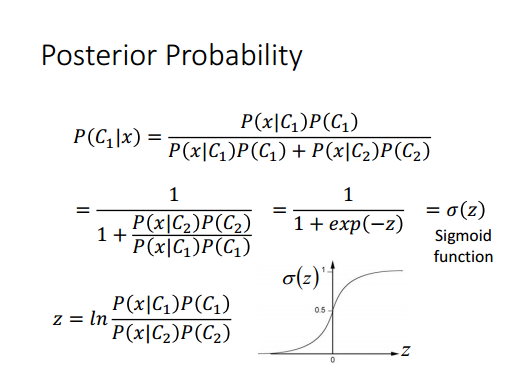
\includegraphics[scale=0.4]{pic/posterior_probability}}\quad
\subcaptionbox{数学机理1}{%
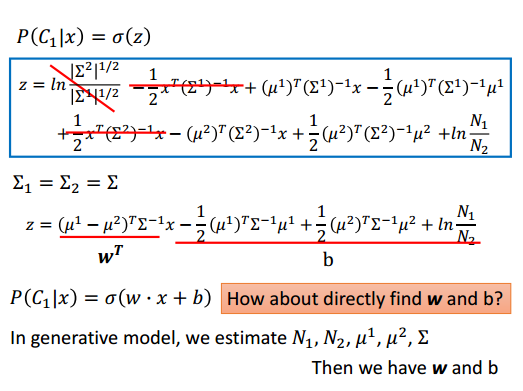
\includegraphics[scale=0.4]{pic/posterior_probability_02}}
}
\caption{生成模型到判别模型数学机理}
\label{fig:math_of_generation model}
\end{figure}

可见,生成模型,通过计算概率的方式,通过特征均值$\mu$和协方差矩阵$\Sigma$,求出合适的$w$ 和$b$,其值和假设的模型分布有关;而判别模型直接学习分布概率$p(C_1|x)$,即直接通过训练数据直接学习参数$w$和$b$。

基本思想是有限样本条件下建立判别函数,不考虑样本的产生模型,直接研究预测模型。典型的判别模型包括线性回归,k近邻,感知级,决策树,支持向量机等。

\subsubsection{生成模型和判别模型的优缺点}
在监督学习中,两种方法各有优缺点,适合于不同条件的学习问题。

\begin{itemize}
	\item 生成方法的特点:上面说到,生成方法学习联合概率密度分布$P(X,Y)$,所以就可以从统计的角度表示数据的分布情况,能够反映同类数据本身的相似度。但它不关心到底划分各类的那个分类边界在哪。生成方法可以还原出联合概率分布$P(Y|X)$,而判别方法不能。生成方法的学习收敛速度更快,即当样本容量增加的时候,学到的模型可以更快的收敛于真实模型,当存在隐变量时,仍可以用生成方法学习。此时判别方法就不能用。
	\item 判别方法的特点:判别方法直接学习的是决策函数$Y=f(X)$或者条件概率分布$P(Y|X)$。不能反映训练数据本身的特性。但它寻找不同类别之间的最优分类面,反映的是异类数据之间的差异。直接面对预测,往往学习的准确率更高。由于直接学习$P(Y|X)$或$P(X)$,可以对数据进行各种程度上的抽象、定义特征并使用特征,因此可以简化学习问题。
	\end{itemize}


\subsubsection{生成模型和判别模型的联系}
由生成模型可以得到判别模型,但由判别模型得不到生成模型。
%[^1]: http://blog.csdn.net/Fishmemory/article/details/51711114
%[^2]: http://blog.csdn.net/zouxy09/article/details/8195017
